\documentclass[]{article}
\usepackage{lmodern}
\usepackage{amssymb,amsmath}
\usepackage{ifxetex,ifluatex}
\usepackage{fixltx2e} % provides \textsubscript
\ifnum 0\ifxetex 1\fi\ifluatex 1\fi=0 % if pdftex
  \usepackage[T1]{fontenc}
  \usepackage[utf8]{inputenc}
\else % if luatex or xelatex
  \ifxetex
    \usepackage{mathspec}
  \else
    \usepackage{fontspec}
  \fi
  \defaultfontfeatures{Ligatures=TeX,Scale=MatchLowercase}
\fi
% use upquote if available, for straight quotes in verbatim environments
\IfFileExists{upquote.sty}{\usepackage{upquote}}{}
% use microtype if available
\IfFileExists{microtype.sty}{%
\usepackage{microtype}
\UseMicrotypeSet[protrusion]{basicmath} % disable protrusion for tt fonts
}{}
\usepackage[margin=1in]{geometry}
\usepackage{hyperref}
\hypersetup{unicode=true,
            pdftitle={Reproducible Research: Peer Assessment 1},
            pdfauthor={Greg Verissimo},
            pdfborder={0 0 0},
            breaklinks=true}
\urlstyle{same}  % don't use monospace font for urls
\usepackage{color}
\usepackage{fancyvrb}
\newcommand{\VerbBar}{|}
\newcommand{\VERB}{\Verb[commandchars=\\\{\}]}
\DefineVerbatimEnvironment{Highlighting}{Verbatim}{commandchars=\\\{\}}
% Add ',fontsize=\small' for more characters per line
\usepackage{framed}
\definecolor{shadecolor}{RGB}{248,248,248}
\newenvironment{Shaded}{\begin{snugshade}}{\end{snugshade}}
\newcommand{\AlertTok}[1]{\textcolor[rgb]{0.94,0.16,0.16}{#1}}
\newcommand{\AnnotationTok}[1]{\textcolor[rgb]{0.56,0.35,0.01}{\textbf{\textit{#1}}}}
\newcommand{\AttributeTok}[1]{\textcolor[rgb]{0.77,0.63,0.00}{#1}}
\newcommand{\BaseNTok}[1]{\textcolor[rgb]{0.00,0.00,0.81}{#1}}
\newcommand{\BuiltInTok}[1]{#1}
\newcommand{\CharTok}[1]{\textcolor[rgb]{0.31,0.60,0.02}{#1}}
\newcommand{\CommentTok}[1]{\textcolor[rgb]{0.56,0.35,0.01}{\textit{#1}}}
\newcommand{\CommentVarTok}[1]{\textcolor[rgb]{0.56,0.35,0.01}{\textbf{\textit{#1}}}}
\newcommand{\ConstantTok}[1]{\textcolor[rgb]{0.00,0.00,0.00}{#1}}
\newcommand{\ControlFlowTok}[1]{\textcolor[rgb]{0.13,0.29,0.53}{\textbf{#1}}}
\newcommand{\DataTypeTok}[1]{\textcolor[rgb]{0.13,0.29,0.53}{#1}}
\newcommand{\DecValTok}[1]{\textcolor[rgb]{0.00,0.00,0.81}{#1}}
\newcommand{\DocumentationTok}[1]{\textcolor[rgb]{0.56,0.35,0.01}{\textbf{\textit{#1}}}}
\newcommand{\ErrorTok}[1]{\textcolor[rgb]{0.64,0.00,0.00}{\textbf{#1}}}
\newcommand{\ExtensionTok}[1]{#1}
\newcommand{\FloatTok}[1]{\textcolor[rgb]{0.00,0.00,0.81}{#1}}
\newcommand{\FunctionTok}[1]{\textcolor[rgb]{0.00,0.00,0.00}{#1}}
\newcommand{\ImportTok}[1]{#1}
\newcommand{\InformationTok}[1]{\textcolor[rgb]{0.56,0.35,0.01}{\textbf{\textit{#1}}}}
\newcommand{\KeywordTok}[1]{\textcolor[rgb]{0.13,0.29,0.53}{\textbf{#1}}}
\newcommand{\NormalTok}[1]{#1}
\newcommand{\OperatorTok}[1]{\textcolor[rgb]{0.81,0.36,0.00}{\textbf{#1}}}
\newcommand{\OtherTok}[1]{\textcolor[rgb]{0.56,0.35,0.01}{#1}}
\newcommand{\PreprocessorTok}[1]{\textcolor[rgb]{0.56,0.35,0.01}{\textit{#1}}}
\newcommand{\RegionMarkerTok}[1]{#1}
\newcommand{\SpecialCharTok}[1]{\textcolor[rgb]{0.00,0.00,0.00}{#1}}
\newcommand{\SpecialStringTok}[1]{\textcolor[rgb]{0.31,0.60,0.02}{#1}}
\newcommand{\StringTok}[1]{\textcolor[rgb]{0.31,0.60,0.02}{#1}}
\newcommand{\VariableTok}[1]{\textcolor[rgb]{0.00,0.00,0.00}{#1}}
\newcommand{\VerbatimStringTok}[1]{\textcolor[rgb]{0.31,0.60,0.02}{#1}}
\newcommand{\WarningTok}[1]{\textcolor[rgb]{0.56,0.35,0.01}{\textbf{\textit{#1}}}}
\usepackage{graphicx,grffile}
\makeatletter
\def\maxwidth{\ifdim\Gin@nat@width>\linewidth\linewidth\else\Gin@nat@width\fi}
\def\maxheight{\ifdim\Gin@nat@height>\textheight\textheight\else\Gin@nat@height\fi}
\makeatother
% Scale images if necessary, so that they will not overflow the page
% margins by default, and it is still possible to overwrite the defaults
% using explicit options in \includegraphics[width, height, ...]{}
\setkeys{Gin}{width=\maxwidth,height=\maxheight,keepaspectratio}
\IfFileExists{parskip.sty}{%
\usepackage{parskip}
}{% else
\setlength{\parindent}{0pt}
\setlength{\parskip}{6pt plus 2pt minus 1pt}
}
\setlength{\emergencystretch}{3em}  % prevent overfull lines
\providecommand{\tightlist}{%
  \setlength{\itemsep}{0pt}\setlength{\parskip}{0pt}}
\setcounter{secnumdepth}{0}
% Redefines (sub)paragraphs to behave more like sections
\ifx\paragraph\undefined\else
\let\oldparagraph\paragraph
\renewcommand{\paragraph}[1]{\oldparagraph{#1}\mbox{}}
\fi
\ifx\subparagraph\undefined\else
\let\oldsubparagraph\subparagraph
\renewcommand{\subparagraph}[1]{\oldsubparagraph{#1}\mbox{}}
\fi

%%% Use protect on footnotes to avoid problems with footnotes in titles
\let\rmarkdownfootnote\footnote%
\def\footnote{\protect\rmarkdownfootnote}

%%% Change title format to be more compact
\usepackage{titling}

% Create subtitle command for use in maketitle
\providecommand{\subtitle}[1]{
  \posttitle{
    \begin{center}\large#1\end{center}
    }
}

\setlength{\droptitle}{-2em}

  \title{Reproducible Research: Peer Assessment 1}
    \pretitle{\vspace{\droptitle}\centering\huge}
  \posttitle{\par}
    \author{Greg Verissimo}
    \preauthor{\centering\large\emph}
  \postauthor{\par}
    \date{}
    \predate{}\postdate{}
  

\begin{document}
\maketitle

\begin{center}\rule{0.5\linewidth}{\linethickness}\end{center}

\hypertarget{overview}{%
\subsection{Overview}\label{overview}}

\hypertarget{assignment}{%
\paragraph{\texorpdfstring{\emph{Assignment:}}{Assignment:}}\label{assignment}}

\emph{It is now possible to collect a large amount of data about
personal movement using activity monitoring devices such as a Fitbit,
Nike Fuelband, or Jawbone Up. These type of devices are part of the
``quantified self'' movement -- a group of enthusiasts who take
measurements about themselves regularly to improve their health, to find
patterns in their behavior, or because they are tech geeks. But these
data remain under-utilized both because the raw data are hard to obtain
and there is a lack of statistical methods and software for processing
and interpreting the data.}

\emph{This assignment makes use of data from a personal activity
monitoring device. This device collects data at 5 minute intervals
through out the day. The data consists of two months of data from an
anonymous individual collected during the months of October and
November, 2012 and include the number of steps taken in 5 minute
intervals each day.}

The raw dataset for this assignment

\begin{itemize}
\tightlist
\item
  Was downloaded from here:
  \href{https://d396qusza40orc.cloudfront.net/repdata\%2Fdata\%2Factivity.zip}{Activity
  monitoring data}
\item
  57KB compressed (.zip) and 351KB uncompressed (.csv)
\item
  There are a total of 17,568 observations contained the dataset
\end{itemize}

The variables included in this dataset are:

\begin{enumerate}
\def\labelenumi{\arabic{enumi}.}
\tightlist
\item
  steps: Number of steps taking in a 5-minute interval (missing values
  are coded as ``NA'')
\item
  date: The date on which the measurement was taken in YYYY-MM-DD format
\item
  interval: Identifier for the 5-minute interval in which measurement
  was taken
\end{enumerate}

\begin{center}\rule{0.5\linewidth}{\linethickness}\end{center}

\hypertarget{loading-and-preprocessing-the-data}{%
\subsection{Loading and preprocessing the
data}\label{loading-and-preprocessing-the-data}}

\hypertarget{assignment-1}{%
\paragraph{\texorpdfstring{\emph{Assignment:}}{Assignment:}}\label{assignment-1}}

\emph{Show any code that is needed to}

\begin{enumerate}
\def\labelenumi{\arabic{enumi}.}
\tightlist
\item
  \emph{Load the data (i.e. - read.csv() ) }\\
\item
  \emph{Process/transform the data (if necessary) into a format suitable
  for your analysis}
\end{enumerate}

First load required libraries:

\begin{Shaded}
\begin{Highlighting}[]
\CommentTok{## Load  libraries}
\KeywordTok{library}\NormalTok{(reshape2)}
\KeywordTok{library}\NormalTok{(ggplot2)}
\KeywordTok{library}\NormalTok{(dplyr)}
\end{Highlighting}
\end{Shaded}

We loaded dataset from .csv file into a dataframe (`activity') using
read.csv()

\begin{Shaded}
\begin{Highlighting}[]
\CommentTok{## read raw dats (.csv file) into dataframe ('activity')}
\NormalTok{activity <-}\StringTok{ }\KeywordTok{read.csv}\NormalTok{(}\StringTok{"./data/activity.csv"}\NormalTok{,}
                     \DataTypeTok{header=}\OtherTok{TRUE}\NormalTok{, }
                     \DataTypeTok{colClasses=}\KeywordTok{c}\NormalTok{(}
                             \StringTok{"numeric"}\NormalTok{,   }\CommentTok{## steps: number of steps taken during 5min sub-interval of a day}
                             \StringTok{"character"}\NormalTok{, }\CommentTok{## date: the specific day of sample 'steps'}
                             \StringTok{"numeric"}    \CommentTok{## interval: the specific 5min sub-interval of sample 'steps'}
\NormalTok{                     )}
\NormalTok{)}
\end{Highlighting}
\end{Shaded}

and then converted variables (date, interval) to factors for later
manipulation:

\begin{Shaded}
\begin{Highlighting}[]
\CommentTok{## convert string ("YYYY-MM-DD") to class 'date' and then to 'factor'}
\NormalTok{activity}\OperatorTok{$}\NormalTok{date <-}\StringTok{ }\KeywordTok{as.factor}\NormalTok{(}\KeywordTok{as.Date}\NormalTok{(activity}\OperatorTok{$}\NormalTok{date, }\DataTypeTok{format=}\StringTok{"%Y-%m-%d"}\NormalTok{))}
\CommentTok{## convert interval to class 'factor'}
\NormalTok{activity}\OperatorTok{$}\NormalTok{interval <-}\StringTok{ }\KeywordTok{as.factor}\NormalTok{(activity}\OperatorTok{$}\NormalTok{interval)}
\KeywordTok{str}\NormalTok{(activity)}
\end{Highlighting}
\end{Shaded}

\begin{verbatim}
## 'data.frame':    17568 obs. of  3 variables:
##  $ steps   : num  NA NA NA NA NA NA NA NA NA NA ...
##  $ date    : Factor w/ 61 levels "2012-10-01","2012-10-02",..: 1 1 1 1 1 1 1 1 1 1 ...
##  $ interval: Factor w/ 288 levels "0","5","10","15",..: 1 2 3 4 5 6 7 8 9 10 ...
\end{verbatim}

\begin{center}\rule{0.5\linewidth}{\linethickness}\end{center}

\hypertarget{what-is-mean-total-number-of-steps-taken-per-day}{%
\subsection{What is mean total number of steps taken per
day?}\label{what-is-mean-total-number-of-steps-taken-per-day}}

\hypertarget{assignment-2}{%
\paragraph{\texorpdfstring{\emph{Assignment:}}{Assignment:}}\label{assignment-2}}

\emph{For this part of the assignment, you can ignore the missing values
in the dataset.}

\begin{enumerate}
\def\labelenumi{\arabic{enumi}.}
\tightlist
\item
  \emph{Calculate the total number of steps taken per day}\\
\item
  \emph{Make a histogram of the total number of steps taken each day. If
  you do not understand the difference between a histogram and a
  barplot, research the difference between them.}\\
\item
  \emph{Calculate and report the mean and median of the total number of
  steps taken per day}
\end{enumerate}

Using aggregate() to reshape the dataset around steps by date in
combination with the function sum(), we added up all the 5 minute
intervals for each day into daily totals over the sample period (10/1/12
to 11/30/12).

We then created a histogram of those daily totals where you can see the
subject most frequently walked between 10,000 and 11,000 steps each day:

\begin{Shaded}
\begin{Highlighting}[]
\NormalTok{stepsPerDay <-}\StringTok{ }\KeywordTok{aggregate}\NormalTok{(steps }\OperatorTok{~}\StringTok{ }\NormalTok{date, }\DataTypeTok{data =}\NormalTok{ activity, }\DataTypeTok{FUN =}\NormalTok{ sum, }\DataTypeTok{na.rm =} \OtherTok{TRUE}\NormalTok{)}
\NormalTok{meanStepsPerDay <-}\StringTok{ }\KeywordTok{format}\NormalTok{(}\KeywordTok{round}\NormalTok{(}\KeywordTok{mean}\NormalTok{(stepsPerDay}\OperatorTok{$}\NormalTok{steps), }\DecValTok{1}\NormalTok{), }
                          \DataTypeTok{scientific=}\OtherTok{FALSE}\NormalTok{, }\DataTypeTok{nsmall=}\DecValTok{1}\NormalTok{, }\DataTypeTok{big.mark=}\StringTok{","}\NormalTok{)}
\NormalTok{medianStepsPerDay <-}\StringTok{ }\KeywordTok{format}\NormalTok{(}\KeywordTok{round}\NormalTok{(}\KeywordTok{median}\NormalTok{(stepsPerDay}\OperatorTok{$}\NormalTok{steps), }\DecValTok{1}\NormalTok{), }
                            \DataTypeTok{scientific=}\OtherTok{FALSE}\NormalTok{, }\DataTypeTok{nsmall=}\DecValTok{1}\NormalTok{, }\DataTypeTok{big.mark=}\StringTok{","}\NormalTok{)}

\CommentTok{## Make a histogram of the total number of steps taken each day. If you do not understand the difference between a histogram and a barplot, research the difference between them.*}
\KeywordTok{par}\NormalTok{(}\DataTypeTok{mfrow=}\KeywordTok{c}\NormalTok{(}\DecValTok{1}\NormalTok{,}\DecValTok{1}\NormalTok{), }\DataTypeTok{mar=}\KeywordTok{c}\NormalTok{(}\DecValTok{4}\NormalTok{,}\DecValTok{4}\NormalTok{,}\DecValTok{4}\NormalTok{,}\DecValTok{2}\NormalTok{), }\DataTypeTok{oma=}\KeywordTok{c}\NormalTok{(}\DecValTok{1}\NormalTok{,}\DecValTok{1}\NormalTok{,}\DecValTok{1}\NormalTok{,}\DecValTok{0}\NormalTok{))}
\NormalTok{histInfo <-}\StringTok{ }\KeywordTok{hist}\NormalTok{(stepsPerDay}\OperatorTok{$}\NormalTok{steps, }
     \DataTypeTok{xlim=}\KeywordTok{c}\NormalTok{(}\DecValTok{0}\NormalTok{,}\DecValTok{25000}\NormalTok{), }\DataTypeTok{breaks =} \DecValTok{25}\NormalTok{,}
     \DataTypeTok{col =} \StringTok{"sky blue"}\NormalTok{, }\DataTypeTok{border =} \StringTok{"white"}\NormalTok{,}
     \DataTypeTok{main=}\StringTok{"Histogram of Total Steps per Day"}\NormalTok{,}
     \DataTypeTok{xlab=}\StringTok{"Steps"}\NormalTok{, }\DataTypeTok{ylab=}\StringTok{"Frequency"}\NormalTok{)}
\end{Highlighting}
\end{Shaded}

\includegraphics{PA1_template_files/figure-latex/unnamed-chunk-4-1.pdf}

\begin{Shaded}
\begin{Highlighting}[]
\NormalTok{histInfo[}\KeywordTok{c}\NormalTok{(}\StringTok{"mids"}\NormalTok{, }\StringTok{"counts"}\NormalTok{)]}
\end{Highlighting}
\end{Shaded}

\begin{verbatim}
## $mids
##  [1]   500  1500  2500  3500  4500  5500  6500  7500  8500  9500 10500
## [12] 11500 12500 13500 14500 15500 16500 17500 18500 19500 20500 21500
## 
## $counts
##  [1]  2  0  1  1  1  2  1  2  5  2 10  6  6  4  2  5  0  1  0  0  1  1
\end{verbatim}

The mean steps/day over the period was 10,766.2 and the median was
10,765.0.

\begin{center}\rule{0.5\linewidth}{\linethickness}\end{center}

\hypertarget{what-is-the-average-daily-activity-pattern}{%
\subsection{What is the average daily activity
pattern?}\label{what-is-the-average-daily-activity-pattern}}

\hypertarget{assignment-3}{%
\paragraph{\texorpdfstring{\emph{Assignment:}}{Assignment:}}\label{assignment-3}}

\begin{enumerate}
\def\labelenumi{\arabic{enumi}.}
\tightlist
\item
  \emph{Make a time series plot (i.e. - type=``l'') of the 5-minute
  interval (x-axis) and the average number of steps taken, averaged
  across all days (y-axis)}\\
\item
  \emph{Which 5-minute interval, on average across all the days in the
  dataset, contains the maximum number of steps?}
\end{enumerate}

Again using aggregate() --this time reshaping the dataset around steps
by 5-min interval-- in combination with the function mean(), we
calculated the mean for each 5min interval over the sample period:

\begin{Shaded}
\begin{Highlighting}[]
\NormalTok{averageSteps <-}\StringTok{ }\KeywordTok{aggregate}\NormalTok{(steps }\OperatorTok{~}\StringTok{ }\NormalTok{interval, }\DataTypeTok{data =}\NormalTok{ activity, mean, }\DataTypeTok{na.rm=}\OtherTok{TRUE}\NormalTok{)}
\NormalTok{maxAverageSteps <-}\StringTok{ }\NormalTok{averageSteps[}\KeywordTok{which.max}\NormalTok{(averageSteps}\OperatorTok{$}\NormalTok{steps), ]}

\KeywordTok{par}\NormalTok{(}\DataTypeTok{mfrow=}\KeywordTok{c}\NormalTok{(}\DecValTok{1}\NormalTok{,}\DecValTok{1}\NormalTok{), }\DataTypeTok{mar=}\KeywordTok{c}\NormalTok{(}\DecValTok{4}\NormalTok{,}\DecValTok{4}\NormalTok{,}\DecValTok{4}\NormalTok{,}\DecValTok{2}\NormalTok{), }\DataTypeTok{oma=}\KeywordTok{c}\NormalTok{(}\DecValTok{1}\NormalTok{,}\DecValTok{1}\NormalTok{,}\DecValTok{1}\NormalTok{,}\DecValTok{0}\NormalTok{))}
\KeywordTok{plot}\NormalTok{(}\KeywordTok{as.numeric}\NormalTok{(}\KeywordTok{as.character}\NormalTok{(averageSteps}\OperatorTok{$}\NormalTok{interval)), averageSteps}\OperatorTok{$}\NormalTok{steps, }
     \DataTypeTok{type =} \StringTok{"l"}\NormalTok{, }
     \DataTypeTok{lwd =} \DecValTok{2}\NormalTok{, }\DataTypeTok{col =} \StringTok{"deep sky blue 2"}\NormalTok{,}
     \DataTypeTok{main =} \StringTok{"Steps per 5min Interval Averaged Across All Days"}\NormalTok{,}
     \DataTypeTok{xlab =} \StringTok{"5-min interval"}\NormalTok{, }\DataTypeTok{ylab =} \StringTok{"Average steps per interval"}\NormalTok{ )}
\end{Highlighting}
\end{Shaded}

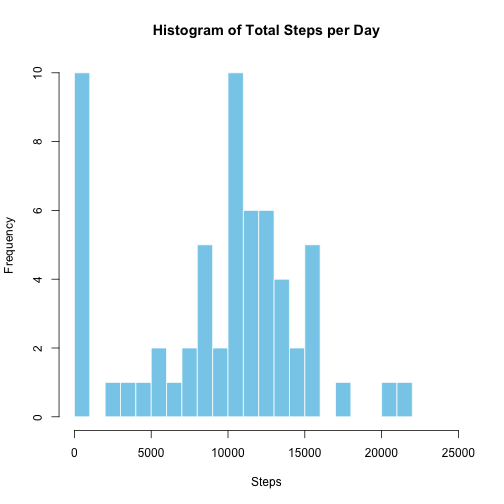
\includegraphics{PA1_template_files/figure-latex/unnamed-chunk-5-1.pdf}

\begin{center}\rule{0.5\linewidth}{\linethickness}\end{center}

\hypertarget{imputing-missing-values}{%
\subsection{Imputing missing values}\label{imputing-missing-values}}

\hypertarget{assignment-4}{%
\paragraph{\texorpdfstring{\emph{Assignment:}}{Assignment:}}\label{assignment-4}}

\emph{Note that there are a number of days/intervals where there are
missing values (coded as NA). The presence of missing days may introduce
bias into some calculations or summaries of the data.}

\begin{enumerate}
\def\labelenumi{\arabic{enumi}.}
\tightlist
\item
  \emph{Calculate and report the total number of missing values in the
  dataset (i.e.~the total number of rows with NAs)}
\item
  \emph{Devise a strategy for filling in all of the missing values in
  the dataset. The strategy does not need to be sophisticated. For
  example, you could use the mean/median for that day, or the mean for
  that 5-minute interval, etc.}
\item
  \emph{Create a new dataset that is equal to the original dataset but
  with the missing data filled in.}
\item
  \emph{Make a histogram of the total number of steps taken each day and
  Calculate and report the mean and median total number of steps taken
  per day.}\\
\end{enumerate}

\begin{itemize}
\tightlist
\item
  \emph{Do these values differ from the estimates from the first part of
  the assignment?}\\
\item
  \emph{What is the impact of imputing missing data on the estimates of
  the total daily number of steps?}
\end{itemize}

Going back to the original dataset, we counted the number of missing
step samples in the dataset

\begin{Shaded}
\begin{Highlighting}[]
\NormalTok{missingValues <-}\StringTok{ }\KeywordTok{sum}\NormalTok{(}\KeywordTok{is.na}\NormalTok{(activity}\OperatorTok{$}\NormalTok{steps))}
\end{Highlighting}
\end{Shaded}

and found there are 2304 missing values. Looking at missing values in
the dataset, we saw the NAs are grouped in terms of entire days.
\textbf{So we decided to impute these missing days with the average day
for the sample period} that we calculated earlier\\
\emph{(ie - by replacing each NA sample interval with the average for
that interval).}

We did this by first reshaping the dataset into wide format
(activityWide) to move the dates (10/1\textasciitilde{}11/30) into
separate columns.

\begin{Shaded}
\begin{Highlighting}[]
\CommentTok{## reshape long->wide to facilitate impute of NAs}
\NormalTok{activityWide <-}\StringTok{ }\KeywordTok{dcast}\NormalTok{(activity, interval }\OperatorTok{~}\StringTok{ }\NormalTok{date, }\DataTypeTok{value.var=}\StringTok{"steps"}\NormalTok{)}
\end{Highlighting}
\end{Shaded}

We then looped over those dates and filtered each date for intervals
containing NA values (`missingVal') and then replacing those missing
values with the corresponding average calculated earlier
(`averageSteps').

\emph{(Note that we also opted to round those imputed values to the
nearest whole step)}

\begin{Shaded}
\begin{Highlighting}[]
\CommentTok{## setup loop variables}
\NormalTok{firstDate <-}\StringTok{ }\KeywordTok{which}\NormalTok{(}\KeywordTok{colnames}\NormalTok{(activityWide)}\OperatorTok{==}\StringTok{"2012-10-01"}\NormalTok{)}
\NormalTok{lastDate <-}\StringTok{ }\KeywordTok{which}\NormalTok{(}\KeywordTok{colnames}\NormalTok{(activityWide)}\OperatorTok{==}\StringTok{"2012-11-30"}\NormalTok{)}
\NormalTok{activityWideImputed <-}\StringTok{ }\NormalTok{activityWide}

\CommentTok{## loop over daterange (Oct/1 to Nov/30)}
\ControlFlowTok{for}\NormalTok{ (i }\ControlFlowTok{in}\NormalTok{ firstDate}\OperatorTok{:}\NormalTok{lastDate) \{}
        \CommentTok{## identify NA's for loop date}
\NormalTok{        missingVal <-}\StringTok{ }\KeywordTok{is.na}\NormalTok{(activityWideImputed[ ,i])}
        \CommentTok{## replace interval NA's with average steps for that interval (rounded to whole steps)}
\NormalTok{        activityWideImputed[missingVal, i] <-}\StringTok{ }\KeywordTok{round}\NormalTok{(averageSteps}\OperatorTok{$}\NormalTok{steps[missingVal],}\DecValTok{0}\NormalTok{)}
\NormalTok{\}}
\end{Highlighting}
\end{Shaded}

We then reshaped the data back to long format (`activityImputed') and
recalculated the average steps per day (`stepsPerDayImputed') and
average steps per 5min interval (averageStepsImputed) -- similar to
above.

\begin{Shaded}
\begin{Highlighting}[]
\CommentTok{## reshape wide->long}
\NormalTok{activityImputed <-}\StringTok{ }\KeywordTok{melt}\NormalTok{(activityWideImputed, }
                        \DataTypeTok{id.vars=}\KeywordTok{c}\NormalTok{(}\StringTok{"interval"}\NormalTok{), }
                        \DataTypeTok{variable.name=}\StringTok{"date"}\NormalTok{,}
                        \DataTypeTok{value.name=}\StringTok{"steps"}\NormalTok{)}

\CommentTok{## Calculate steps per day (imputed NA)}
\NormalTok{stepsPerDayImputed <-}\StringTok{ }\KeywordTok{aggregate}\NormalTok{(steps }\OperatorTok{~}\StringTok{ }\NormalTok{date, }\DataTypeTok{data =}\NormalTok{ activityImputed, sum, }\DataTypeTok{na.rm =} \OtherTok{TRUE}\NormalTok{)}
\NormalTok{averageStepsImputed <-}\StringTok{ }\KeywordTok{aggregate}\NormalTok{(steps }\OperatorTok{~}\StringTok{ }\NormalTok{interval, }\DataTypeTok{data =}\NormalTok{ activityImputed, mean, }\DataTypeTok{na.rm=}\OtherTok{TRUE}\NormalTok{)}
\end{Highlighting}
\end{Shaded}

\begin{center}\rule{0.5\linewidth}{\linethickness}\end{center}

\hypertarget{make-a-histogram-of-the-total-number-of-steps-taken-each-day.-if-you-do-not-understand-the-difference-between-a-histogram-and-a-barplot-research-the-difference-between-them.}{%
\subsection{Make a histogram of the total number of steps taken each
day. If you do not understand the difference between a histogram and a
barplot, research the difference between
them.*}\label{make-a-histogram-of-the-total-number-of-steps-taken-each-day.-if-you-do-not-understand-the-difference-between-a-histogram-and-a-barplot-research-the-difference-between-them.}}

For comparison, we plotted both average daily steps as well as a
histogram of steps/day and unimputed and imputed:

\begin{Shaded}
\begin{Highlighting}[]
\KeywordTok{par}\NormalTok{(}\DataTypeTok{mfrow=}\KeywordTok{c}\NormalTok{(}\DecValTok{1}\NormalTok{,}\DecValTok{2}\NormalTok{), }\DataTypeTok{mar=}\KeywordTok{c}\NormalTok{(}\DecValTok{4}\NormalTok{,}\DecValTok{4}\NormalTok{,}\DecValTok{4}\NormalTok{,}\DecValTok{2}\NormalTok{), }\DataTypeTok{oma=}\KeywordTok{c}\NormalTok{(}\DecValTok{1}\NormalTok{,}\DecValTok{1}\NormalTok{,}\DecValTok{1}\NormalTok{,}\DecValTok{0}\NormalTok{))}

\KeywordTok{plot}\NormalTok{(}\KeywordTok{as.numeric}\NormalTok{(}\KeywordTok{as.character}\NormalTok{(averageSteps}\OperatorTok{$}\NormalTok{interval)), averageSteps}\OperatorTok{$}\NormalTok{steps, }
     \DataTypeTok{type =} \StringTok{"l"}\NormalTok{, }
     \DataTypeTok{lwd =} \DecValTok{2}\NormalTok{, }\DataTypeTok{col =} \StringTok{"deep sky blue 2"}\NormalTok{,}
     \DataTypeTok{main =} \StringTok{"Average Steps/Interval }\CharTok{\textbackslash{}n}\StringTok{"}\NormalTok{,}
     \DataTypeTok{xlab =} \StringTok{"5-min interval"}\NormalTok{, }\DataTypeTok{ylab =} \StringTok{"Number of Steps/Interval"}\NormalTok{ )}
\KeywordTok{plot}\NormalTok{(}\KeywordTok{as.numeric}\NormalTok{(}\KeywordTok{as.character}\NormalTok{(averageStepsImputed}\OperatorTok{$}\NormalTok{interval)), averageStepsImputed}\OperatorTok{$}\NormalTok{steps, }
     \DataTypeTok{type =} \StringTok{"l"}\NormalTok{, }
     \DataTypeTok{lwd =} \DecValTok{2}\NormalTok{, }\DataTypeTok{col =} \StringTok{"deep sky blue 2"}\NormalTok{,}
     \DataTypeTok{main =} \StringTok{"Average Steps/Interval }\CharTok{\textbackslash{}n}\StringTok{(imputed)"}\NormalTok{,}
     \DataTypeTok{xlab =} \StringTok{"5-min interval"}\NormalTok{, }\DataTypeTok{ylab =} \StringTok{"Number of Steps/Interval"}\NormalTok{ )}
\end{Highlighting}
\end{Shaded}

\includegraphics{PA1_template_files/figure-latex/unnamed-chunk-10-1.pdf}

\begin{Shaded}
\begin{Highlighting}[]
\KeywordTok{hist}\NormalTok{(stepsPerDay}\OperatorTok{$}\NormalTok{steps, }
     \DataTypeTok{xlim=}\KeywordTok{c}\NormalTok{(}\DecValTok{0}\NormalTok{,}\DecValTok{25000}\NormalTok{), }\DataTypeTok{breaks =} \DecValTok{25}\NormalTok{,}
     \DataTypeTok{ylim=}\KeywordTok{c}\NormalTok{(}\DecValTok{0}\NormalTok{,}\DecValTok{20}\NormalTok{),}
     \DataTypeTok{col =} \StringTok{"sky blue"}\NormalTok{, }\DataTypeTok{border =} \StringTok{"white"}\NormalTok{,}
     \DataTypeTok{main=}\StringTok{"Histogram of Total Steps/Day }\CharTok{\textbackslash{}n}\StringTok{"}\NormalTok{,}
     \DataTypeTok{xlab=}\StringTok{"Number of Steps/Day"}\NormalTok{, }\DataTypeTok{ylab=}\StringTok{"Frequency"}\NormalTok{)}
\KeywordTok{hist}\NormalTok{(stepsPerDayImputed}\OperatorTok{$}\NormalTok{steps, }
     \DataTypeTok{xlim=}\KeywordTok{c}\NormalTok{(}\DecValTok{0}\NormalTok{,}\DecValTok{25000}\NormalTok{), }\DataTypeTok{breaks =} \DecValTok{25}\NormalTok{,}
     \DataTypeTok{ylim=}\KeywordTok{c}\NormalTok{(}\DecValTok{0}\NormalTok{,}\DecValTok{20}\NormalTok{),}
     \DataTypeTok{col =} \StringTok{"sky blue"}\NormalTok{, }\DataTypeTok{border =} \StringTok{"white"}\NormalTok{,}
     \DataTypeTok{main=}\StringTok{"Histogram of Total Steps/Day }\CharTok{\textbackslash{}n}\StringTok{(imputed)"}\NormalTok{,}
     \DataTypeTok{xlab=}\StringTok{"Number of Steps/Day"}\NormalTok{, }\DataTypeTok{ylab=}\StringTok{"Frequency"}\NormalTok{)}
\end{Highlighting}
\end{Shaded}

\includegraphics{PA1_template_files/figure-latex/unnamed-chunk-10-2.pdf}

\begin{Shaded}
\begin{Highlighting}[]
\NormalTok{meanStepsPerDayImputed <-}\StringTok{ }\KeywordTok{format}\NormalTok{(}\KeywordTok{round}\NormalTok{(}\KeywordTok{mean}\NormalTok{(stepsPerDayImputed}\OperatorTok{$}\NormalTok{steps), }\DecValTok{1}\NormalTok{), }
                          \DataTypeTok{scientific=}\OtherTok{FALSE}\NormalTok{, }\DataTypeTok{nsmall=}\DecValTok{1}\NormalTok{, }\DataTypeTok{big.mark=}\StringTok{","}\NormalTok{)}
\NormalTok{medianStepsPerDayImputed <-}\StringTok{ }\KeywordTok{format}\NormalTok{(}\KeywordTok{round}\NormalTok{(}\KeywordTok{median}\NormalTok{(stepsPerDayImputed}\OperatorTok{$}\NormalTok{steps), }\DecValTok{1}\NormalTok{), }
                            \DataTypeTok{scientific=}\OtherTok{FALSE}\NormalTok{, }\DataTypeTok{nsmall=}\DecValTok{1}\NormalTok{, }\DataTypeTok{big.mark=}\StringTok{","}\NormalTok{)}
\end{Highlighting}
\end{Shaded}

Imputing NAs as described above, the mean \& median statistics changed
very little:

\begin{itemize}
\tightlist
\item
  mean: 10,765.6 (vs.~10,766.2 unimputed)\\
\item
  median: 10,765.6 (vs.~10,765.0unimputed)
\end{itemize}

We attribute this to there being (1) just 8 missing days (out of 61) and
(2) we subsititued average days for the missing ones (which would only
strengthen the mean).

It is interesting to note (again, because we're imputing the average day
for the missing days) that the the only change to the histogram was to
heighten the central peak --which is to be expected.

\begin{center}\rule{0.5\linewidth}{\linethickness}\end{center}

\hypertarget{are-there-differences-in-activity-patterns-between-weekdays-and-weekends}{%
\subsection{Are there differences in activity patterns between weekdays
and
weekends?}\label{are-there-differences-in-activity-patterns-between-weekdays-and-weekends}}

\hypertarget{assignment-5}{%
\paragraph{\texorpdfstring{\emph{Assignment:}}{Assignment:}}\label{assignment-5}}

\emph{For this part the weekdays() function may be of some help here.
Use the dataset with the filled-in missing values for this part.}

\begin{enumerate}
\def\labelenumi{\arabic{enumi}.}
\tightlist
\item
  \emph{Create a new factor variable in the dataset with two levels --
  ``weekday'' and ``weekend'' indicating whether a given date is a
  weekday or weekend day.}
\item
  \emph{Make a panel plot containing a time series plot (i.e. -
  type=``l'') of the 5-minute interval (x-axis) and the average number
  of steps taken, averaged across all weekday days or weekend days
  (y-axis). See the README file in the GitHub repository to see an
  example of what this plot should look like using simulated data.}
\end{enumerate}

With the hint to consider the weekday() function, it was pretty
straightfoward to add a 2-level factor (``Weekend'', ``Weekday'') which
we implemented with a simple: \textbf{IF} (saturday\textbar{}sunday)
\textbf{THEN} weekend \textbf{ELSE} weekday

\begin{Shaded}
\begin{Highlighting}[]
\NormalTok{activityImputed2 <-}\StringTok{ }\NormalTok{activityImputed}
\NormalTok{activityImputed2}\OperatorTok{$}\NormalTok{weekDayEnd <-}\StringTok{ }\KeywordTok{ifelse}\NormalTok{(}\KeywordTok{weekdays}\NormalTok{(}\KeywordTok{as.Date}\NormalTok{(activityImputed2}\OperatorTok{$}\NormalTok{date)) }\OperatorTok\StringTok{ }\KeywordTok{c}\NormalTok{(}\StringTok{"Saturday"}\NormalTok{, }\StringTok{"Sunday"}\NormalTok{),}\StringTok{"Weekend"}\NormalTok{, }\StringTok{"Weekday"}\NormalTok{ )}
\NormalTok{activityImputed2}\OperatorTok{$}\NormalTok{weekDayEnd <-}\StringTok{ }\KeywordTok{as.factor}\NormalTok{(activityImputed2}\OperatorTok{$}\NormalTok{weekDayEnd)}
\end{Highlighting}
\end{Shaded}

And then reshaped the data around steps by interval (similar to above)
and created the comparison plot using ggplot:

\begin{Shaded}
\begin{Highlighting}[]
\NormalTok{stepsPerDayImputed2 <-}\StringTok{ }\KeywordTok{aggregate}\NormalTok{(steps }\OperatorTok{~}\StringTok{ }\NormalTok{interval }\OperatorTok{+}\StringTok{ }\NormalTok{weekDayEnd, activityImputed2, mean)}

\NormalTok{pl <-}\StringTok{ }\KeywordTok{ggplot}\NormalTok{(}\KeywordTok{filter}\NormalTok{(stepsPerDayImputed2, weekDayEnd }\OperatorTok\StringTok{ }\KeywordTok{c}\NormalTok{(}\StringTok{"Weekend"}\NormalTok{, }\StringTok{"Weekday"}\NormalTok{)),}
             \KeywordTok{aes}\NormalTok{(}\DataTypeTok{x=}\KeywordTok{as.numeric}\NormalTok{(}\KeywordTok{as.character}\NormalTok{(interval)), }\DataTypeTok{y=}\NormalTok{steps, }\DataTypeTok{color=}\NormalTok{weekDayEnd) ) }\OperatorTok{+}
\StringTok{        }\KeywordTok{geom_line}\NormalTok{() }\OperatorTok{+}
\StringTok{        }\KeywordTok{facet_grid}\NormalTok{(weekDayEnd }\OperatorTok{~}\StringTok{ }\NormalTok{., }\DataTypeTok{scales=}\StringTok{"fixed"}\NormalTok{, }\DataTypeTok{space=}\StringTok{"fixed"}\NormalTok{) }\OperatorTok{+}
\StringTok{        }\KeywordTok{labs}\NormalTok{(}\DataTypeTok{x=}\StringTok{"interval"}\NormalTok{, }
             \DataTypeTok{y=}\StringTok{"number of steps/day"}\NormalTok{,}
             \DataTypeTok{color=} \StringTok{"Part of Week"}\NormalTok{,}
             \DataTypeTok{title=}\StringTok{"Average Steps/Interval"}\NormalTok{,}
             \DataTypeTok{subtitle=}\StringTok{"Comparison of Weekends vs. Weekdays"}
\NormalTok{             ) }\OperatorTok{+}
\StringTok{        }\KeywordTok{theme}\NormalTok{(}
                \DataTypeTok{legend.position =} \StringTok{"none"}\NormalTok{,}
                \DataTypeTok{plot.margin =} \KeywordTok{unit}\NormalTok{(}\KeywordTok{c}\NormalTok{(}\FloatTok{1.5}\NormalTok{,}\DecValTok{1}\NormalTok{,}\FloatTok{1.5}\NormalTok{,}\DecValTok{1}\NormalTok{), }\StringTok{"cm"}\NormalTok{),}
                \DataTypeTok{strip.text.y =} \KeywordTok{element_text}\NormalTok{(}\DataTypeTok{face=}\StringTok{"bold"}\NormalTok{)}
\NormalTok{                )}
\KeywordTok{print}\NormalTok{(pl)}
\end{Highlighting}
\end{Shaded}

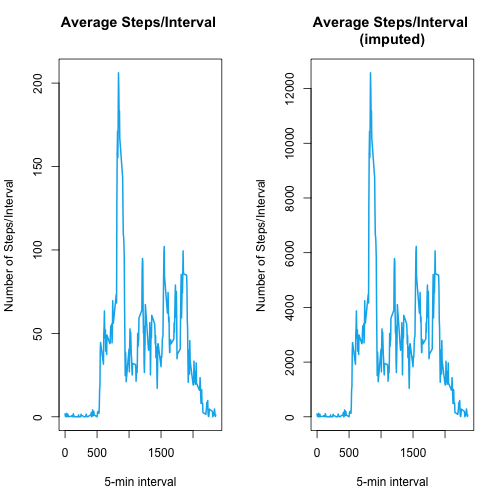
\includegraphics{PA1_template_files/figure-latex/unnamed-chunk-12-1.pdf}

From the plots we observed the following:

\begin{itemize}
\tightlist
\item
  on the weekend start-of-day activity is much lower and ramps more
  gradually

  \begin{itemize}
  \tightlist
  \item
    \ldots{}and the morning peak (around 800) is lower \emph{(our guess:
    no commute)}\\
  \end{itemize}
\item
  on the weekend mid-day activity is significantly higher (roughly twice
  as high compared to weekdays)\\
\item
  on the weekend there is a gradual rolloff at end-of-dayroll

  \begin{itemize}
  \tightlist
  \item
    \ldots{}with no peak (around 1800) \emph{(our guess: no commute)}
  \end{itemize}
\end{itemize}


\end{document}
